%%% Local Variables:
%%% TeX-master: "slides"
%%% End:


% \begin{frame}{The Modern Text Generation Challenge}
%   \begin{center}
% \begin{tikzpicture}
% \node{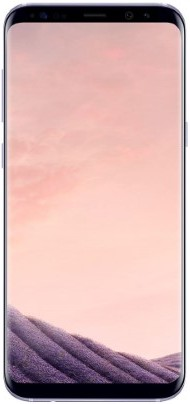
\includegraphics[width=5cm]{galaxy}};
% \end{tikzpicture}
%   \end{center}
% \end{frame}

% \begin{frame}{Machine Learning for Multiclass Prediction}
%   \[ {y} = g({x}; {\theta}) \]
% \end{frame}

\begin{frame}{Machine Learning for Multiclass Classification}


  \begin{center}
    \begin{tikzpicture}
      \node(a) [rectangle,  xshift=-5cm, scale=0.6, draw,thick,fill=blue!0, rounded corners, inner sep =5pt] {
        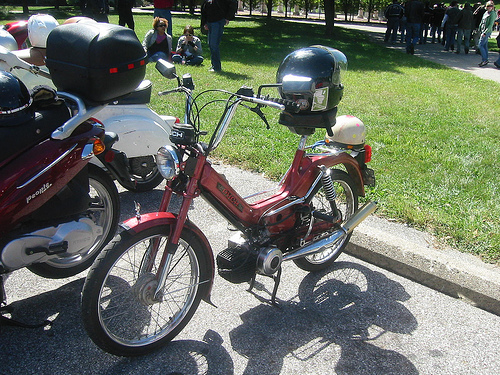
\includegraphics[width=7cm]{moped}};
      \node [rounded corners, above =(0.2cm) of a] {$x$};


      \visible<2->{
      \node(gal){
\includegraphics[width=1.5cm]{phone}};
      \node [rounded corners, above =(0.2cm) of gal] {${\theta}$};
\path[draw, ->] (a) --  (a -|  gal.west) ;
    }



\visible<3->{

  \node (b) [xshift=4.2cm, rectangle, draw,thick,fill=blue!0,text width=8em, rounded corners, inner sep =5pt, minimum height=1em, text centered]{\baselineskip=50pt  \centering Moped};
  \node [rounded corners, above = (0.2cm) of b] {{$y$}};
  \path[draw, <-] (b) --  (b -| gal.east);
  }

\end{tikzpicture}
\end{center}
\note{If you have seen any problem in machine learning, its probably multiclass prediction. Here we are given an input x, which is passed to a model g, to predict a label y. The model's parameters $\theta$
are set by looking at a large set of labeled examples. A major story in the last decade of machine learning has been the improvement of these types of tasks based on deep learning models. Deep learning
here describes the form and structure of the model g and its parameters theta.   }
\end{frame}


\begin{frame}{Machine Learning for Text Generation}

  \[ \alert<3>{y^*_{1:T}} = \argmax_{y_{\tikzmark{opt}1:T}} \alert<4>{\theta}(\alert<3>{y_{1:T}}, \tikzmark{input}\alert<2>{x}; \tikzmark{nn}\alert<4>{\theta}) \]

% \begin{tikzpicture}[
%   remember picture,
%   overlay]

% \node (ptdex) [below left=  of {pic cs:pd}] {Output};
% \node (ptdexa) [below right =  of {pic cs:nn}] {Neural Network};
% \node (ptdexb) [below = of {pic cs:opt}] {Optimization};
% \node (ptdexc) [below = of {pic cs:input}] {Input};
% \draw[->] (ptdex.north) -- ({pic cs:pd});
% \draw[->] (ptdexa.north) -- ({pic cs:nn});
% \draw[->] (ptdexb.north) -- ({pic cs:opt});
% \draw[->] (ptdexc.north) -- ({pic cs:input});
% \end{tikzpicture}

  \begin{itemize}
    \pause
  \item Input \alert<2>{$x$},  \textit{what to talk about}
    \air
    \pause
  \item Output text \alert<3>{$y^*_{1:T}$}, \textit{how to say it}
    \air
    \pause
  \item Model \alert<4>{$f(.; \theta)$}, learned from data
  \end{itemize}
\end{frame}


% \begin{frame}{Part 1: Generating Text}
%   \begin{center}
%     \begin{tikzpicture}
%       \node[draw, fill=yellow, thick, rounded corners] (app) at (0mm,
%       0mm) {Applications};
%     \end{tikzpicture}
%   \end{center}
% \end{frame}


\begin{frame}{Machine Translation}
  \begin{center}
    \begin{tikzpicture}

      \node (gal) {
\includegraphics[width=1.5cm]{phone}};
      \node [rounded corners, above =(0.2cm) of gal] {$f$};

      \node (a) [rectangle, yshift=1cm, xshift=-5cm, scale=0.8, draw,thick,fill=blue!0,text width=16em, rounded corners, inner sep =5pt, minimum height=1em] {
        Yalitza Aparicio acababa de graduarse de una escuela para maestros y aun no tenia empleo cuando el proceso de busqueda de actrices para la ultima pelicula de Alfonso Cuaron llego a su natal Tlaxiaco, Oaxaca.
};
      \path[draw, ->] (a) --  (a -|  gal.west) ;


      \node [rounded corners, above =(0.2cm) of a] {\alert<1>{$x$}};

      \visible<2>{
        \node(b) [xshift=4.5cm, yshift=-1cm, rectangle, scale=0.8, draw,thick,fill=blue!0,text width=12em, rounded corners, inner sep =5pt, minimum height=1em]{\baselineskip=50pt \small
          Yalitza Aparicio had just finished her teaching degree and didn't yet have a job when the Mexican director Alfonso Cuaron held a casting call in her home of Tlaxiaco, Oaxaca, for the lead role in his semi-autobiographical drama, ``Roma.''
          \par};

        \node [rounded corners, above = (0.2cm) of b] {\alert<2>{$y^*_{1:T}$}};
        \path[draw, <-] (b) --  (b -| gal.east) ;
      }
    \end{tikzpicture}
  \end{center}
\end{frame}


\begin{frame}{Translation Performance}


\textbf{Evaluation Metric:}

Target:\  \
\texttt{[Yalitza Aparicio had] just [finished her] teaching [degree] .}
\air

Predict:
\texttt{[Yalitza Aparicio had] recently [finished her] [degree]. }
\pause

\air
\textbf{Deep Learning Performance:}
  \begin{center}
     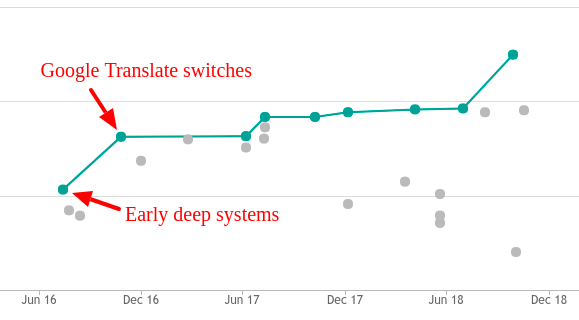
\includegraphics[width=8cm]{wmt}
  \end{center}
\end{frame}

\begin{frame}{Sentence Summarization }
  \begin{center}
    \begin{tikzpicture}

      \node (gal) {
\includegraphics[width=1.5cm]{phone}};
      \node [rounded corners, above =(0.2cm) of gal] {$f$};


      \node (a) [rectangle, yshift=1cm, xshift=-5cm, scale=0.8, draw,thick,fill=blue!0,text width=20em, rounded corners, inner sep =5pt, minimum height=1em] {
        \small
        Cambodian leader Hun Sen on friday rejected opposition parties' demands for talks outside the country, accusing them of trying to ``internationalize'' the political crisis.};
      \path<2>[draw, ->] (a) --  (a -|  gal.west) ;


      \node [rounded corners, above =(0.2cm) of a] {\alert<1>{$x$}};

      \visible<2>{
        \node(b) [xshift=4.5cm, yshift=-1cm, rectangle, scale=0.8, draw,thick,fill=blue!0,text width=12em, rounded corners, inner sep =5pt, minimum height=1em]{\baselineskip=50pt \small
          Cambodian government rejects opposition's call for talks abroad
          \par};

        \node [rounded corners, above = (0.2cm) of b] {\alert<2>{$y_{1:T}$}};
        \path[draw, <-] (b) --  (b -| gal.east) ;
      }
    \end{tikzpicture}
  \end{center}
\end{frame}


\begin{frame}{GigaWord Dataset}
  \research{\citet{Rush2015} w/ Facebook}

  \begin{center}
    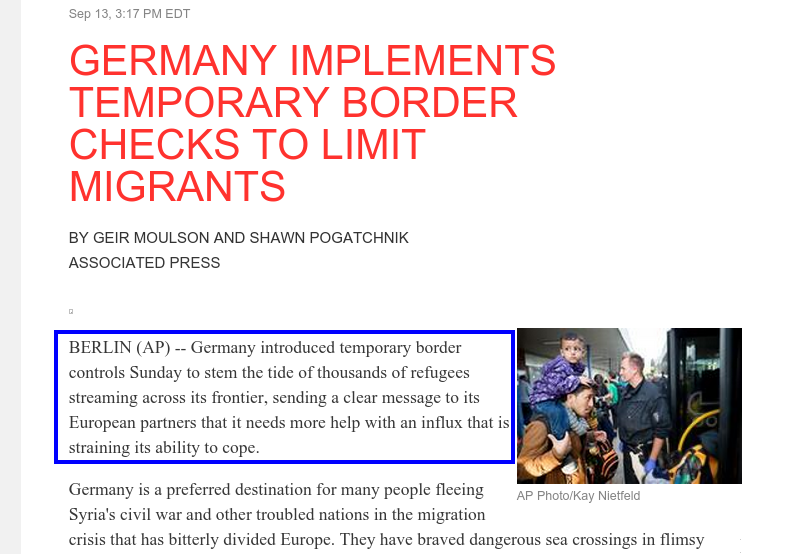
\includegraphics[width=7cm]{ap}
  \end{center}
  \begin{itemize}
  \item Several million headlines paired with article leads.
  \item Model for  abstractive summarization / compression.
  \end{itemize}
\end{frame}



\begin{frame}{Sentence Summarization}
  \begin{center}
    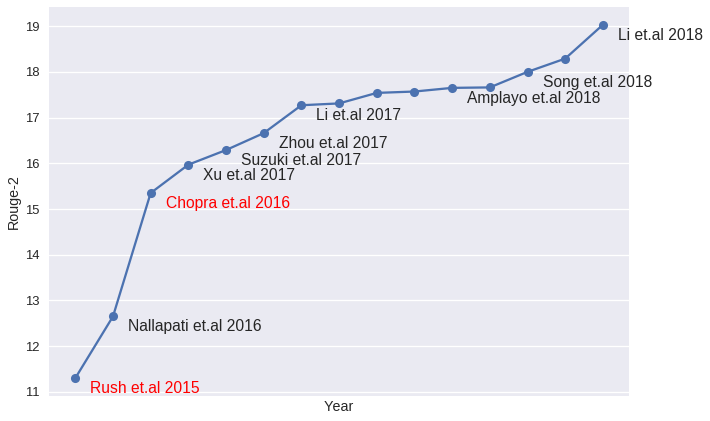
\includegraphics[height=0.75\textheight]{Gigaword}
  \end{center}
\end{frame}

% \begin{frame}{Document Summary}
%   \begin{center}
%     \begin{tikzpicture}
%       \node{
\includegraphics[width=1.5cm]{phone}};
%       \node(a) [rectangle, yshift=0.2cm, xshift=-5cm, scale=0.6, draw,thick,fill=blue!0,text width=25em, rounded corners, inner sep =5pt, minimum height=1em] {
%         \small
%         London, England  (reuters) -- Harry Potter star Daniel Radcliffe gains access to a reported \$20 million fortune as he turns 18 on monday, but he insists the money won't  cast a spell on him. Daniel Radcliffe as harry potter in ``Harry Potter and the Order of the Phoenix'' to the disappointment of gossip columnists around the world , the young actor says he has no plans to fritter his cash away on fast cars , drink and celebrity parties . `` i do n't plan to be one of those people who , as soon as they turn 18 , suddenly buy themselves a massive sports car collection or something similar , '' he told an australian interviewer earlier this month . `` i do n't think i 'll be particularly extravagant '' . `` the things i like buying are things that cost about 10 pounds -- books and cds and dvds . '' at 18 , radcliffe will be able to gamble in a casino , buy a drink in a pub or see the horror film `` hostel : part ii , '' currently six places below his number one movie on the uk box office chart  . details of how he 'll mark his landmark birthday are under wraps . his agent and publicist had no comment on his plans . `` i 'll definitely have some sort of party , '' he said in an interview $\ldots$ %`` hopefully none of you will be reading about it . '' radcliffe 's earnings from the first five potter films have been held in a trust fund which he has not been able to touch . despite his growing fame and riches , the actor says he is keeping his feet firmly on the ground . `` people are always $\ldots$
% };

% \path[draw, ->] (a) --  (a -|  gal.west) ;

% \visible<2>{
%   \node (b) [xshift=4.2cm, yshift=-0.2cm, rectangle, scale=0.8, draw,thick,fill=blue!0,text width=12em, rounded corners, inner sep =5pt, minimum height=1em]{\baselineskip=50pt \footnotesize
%     Harry Potter star Daniel Radcliffe gets \$20m fortune as he turns 18 monday. Young actor says he has no plans to fritter his cash away. Radcliffe 's earnings from first five potter films have been held in trust fund.  \par};
%   \path[draw, <-] (b) --  (b -| gal.east);
%   }

% \end{tikzpicture}
% \end{center}
% \end{frame}


% \begin{frame}{Document Summarization}
%   \begin{center}
%     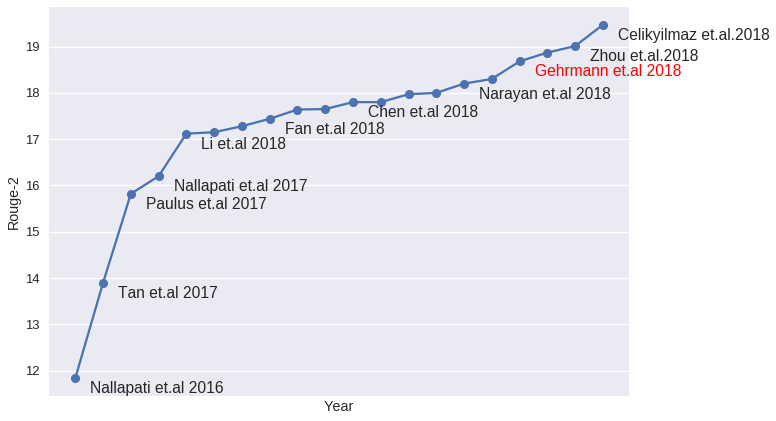
\includegraphics[height=0.75\textheight]{CNNDM}
%   \end{center}
% \end{frame}


\begin{frame}{Talk about Data }

  \research{\cite{EMNLP2017}}
  \begin{center}
\begin{tikzpicture}
\node[]{
\includegraphics[width=1.5cm]{phone}};

\node(a)[xshift=-4.5cm, draw, scale=0.5, inner sep=10pt, rounded corners, text width=26em]{
\small
  \begin{center}

\begin{tabular}{lcccccc}
\toprule
{} & WIN & LOSS & PTS & FG\_PCT & RB & AS \ldots \\
TEAM &           &             &          &             &          &          \\
\midrule
Heat      &        11 &          12 &      103 &          49 &       47 &       27 \\
Hawks     &         7 &          15 &       95 &          43 &       33 &       20 \\
\bottomrule
\end{tabular}
\vspace{0.5cm}

\begin{tabular}{lccccccccc}
\toprule
{} &  AS &    RB &   PT &  FG &  FGA & CITY  $\ldots$ \\
PLAYER      &      &      &      &       &      &      &           \\
\midrule
Tyler Johnson    &    5 &    2 &  27 &    8 &   16 &     Miami \\
Dwight Howard    &    11 &    17 &  23 &    9 &   11 &   Atlanta \\
Paul Millsap     &    2 &    9 &  21 &    8 &   12 &   Atlanta \\
Goran Dragic     &    4 &    2 &  21 &    8 &   17 &     Miami \\
Wayne Ellington  &    2 &    3 &  19 &    7 &   15 &     Miami \\
Dennis Schroder  &    7 &    4 &  17 &    8 &   15 &   Atlanta \\
Rodney McGruder  &    5 &    5 &  11 &    3 &    8 &     Miami \\
\ldots \\
\bottomrule
\end{tabular}
  \end{center}
};

\path[draw, ->] (a) --  (a -|  gal.west) ;


% \node[inner sep=1pt, rounded corners, text width=15em, xshift=-4cm,]{\small
%   \begin{center}
% \vspace{0.5cm}
% \footnotesize
% \begin{tabular}{lcccccc}
% \toprule
% {} & W & L & PTS &  \ldots \\
% TEAM &           &             &          &                      \\
% \midrule
% Heat   &        11 &          12 &      103 &     \ldots      \\
% Hawks  &         7 &          15 &       95 &     \ldots      \\
% \bottomrule

% \vspace*{0.3cm}
% \end{tabular}

% % \begin{tabular}{lccccccccc}
% % \toprule
% % {} &  AS &    RB &   PT &  FG &  FGA & CITY  $\ldots$ \\
% % PLAYER      &      &      &      &       &      &      &           \\
% % \midrule
% % Tyler Johnson    &    5 &    2 &  27 &    8 &   16 &     Miami \\
% % Dwight Howard    &    11 &    17 &  23 &    9 &   11 &   Atlanta \\
% % Paul Millsap     &    2 &    9 &  21 &    8 &   12 &   Atlanta \\
% % Goran Dragic     &    4 &    2 &  21 &    8 &   17 &     Miami \\
% % Wayne Ellington  &    2 &    3 &  19 &    7 &   15 &     Miami \\
% % Dennis Schroder  &    7 &    4 &  17 &    8 &   15 &   Atlanta \\
% % Rodney McGruder  &    5 &    5 &  11 &    3 &    8 &     Miami \\
% % \ldots \\
% % \bottomrule
% % \end{tabular}

%   \end{center}




% };
 % \node [xshift=-3.5cm, rectangle, draw,thick,fill=blue!0,text width=8em, rounded corners, inner sep =5pt, minimum height=1em]{\baselineskip=50pt \footnotesize The Atlanta Hawks defeated the Miami Heat, 103 - 95, at Philips Arena on Wednesday. Atlanta  ... \par};
\visible<2>{\node(b) [xshift=4.5cm,scale=0.5,  rectangle, draw,thick,fill=blue!0,text width=26em, rounded corners, inner sep =10pt, minimum height=1em]{\baselineskip=100pt \large  The Atlanta Hawks defeated the Miami Heat, 103 - 95, at Philips Arena on Wednesday. Atlanta was in desperate need of a win and they were able to take care of a shorthanded Miami team here. Defense was key for the Hawks, as they held the Heat to 42 percent shooting and forced them to commit 16 turnovers. Atlanta also dominated in the paint, winning the rebounding battle, 47 - 34, and outscoring them in the paint 58 - 26. The Hawks shot 49 percent from the field and assisted on 27 of their 43 made baskets. This was a near wire-to-wire win for the Hawks, as Miami held just one lead in the first five minutes. Miami ( 7 - 15 ) are as beat-up as anyone right now and it's taking a toll on the heavily used starters. Hassan Whiteside really struggled in this game, as he amassed eight points, 12 rebounds and one blocks on 4 - of - 12 shooting ... \par};

  \path[draw, <-] (b) --  (b -| gal.east);
}
% \visible<2>{\node[xshift=3.5cm, rectangle, draw,thick,fill=blue!0,text width=8em, rounded corners, inner sep =5pt, minimum height=1em]{\baselineskip=50pt \footnotesize The Atlanta Hawks defeated the Miami Heat, 103 - 95, at Philips Arena on Wednesday. Atlanta  ... \par};}
\end{tikzpicture}
  \end{center}
\end{frame}




\begin{myverbbox}{\sTWO}
 { \cal K } ^ { L } ( \sigma = 2 ) = \left( \begin{array}
{ c c } { - \frac { d ^ { 2 } } { d x ^ { 2 } } + 4 - \frac
 { 3 } { \operatorname { c o s h } ^ { 2 } x } } \& { \frac
 { 3 } { d x ^ { 2 } } }  { \frac { 3 } { \operatorname
 { c o s h } ^ { 2 } x } } \& { - \frac { d ^ { 2 } }
{ d x ^ { 2 } } + 4 - \frac { 3 } { \operatorname { c o s h }
^ { 2 } x } }  \end{array} \right) \qquad
\end{myverbbox}

% \begin{frame}{E2E Challenge 2018}
%   \begin{figure}
%     \centering

%     \footnotesize
% \begin{tabular}{@{}ll@{}}
% \toprule
% \bf MR        & \begin{tabular}[c]{@{}l@{}}name{[}The Golden Palace{]},  eatType{[}coffee shop{]},  food{[}Fast food{]}, \\ priceRange{[}cheap{]},  customer rating{[}5 out of 5{]},  area{[}riverside{]}\end{tabular}         \\ \midrule
% \bf Reference & \begin{tabular}[c]{@{}l@{}}A coffee shop located on the riverside  called The Golden Palace,  \\ has a 5 out of 5 customer rating.  Its price range are fairly cheap  \\for its excellent Fast food.\end{tabular} \\ \bottomrule
% \end{tabular}
%   \end{figure}
%   \begin{center}
%     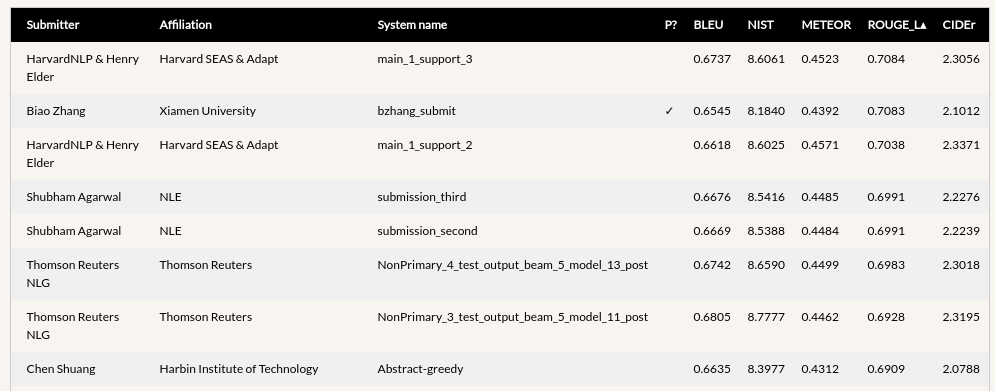
\includegraphics[width=\textwidth]{E2EChallenge}
%   \end{center}
% \end{frame}



\begin{frame}{Talk about the Diagrams}
\research{\cite{Deng2016} w/ Bloomberg}
  \begin{center}
\begin{tikzpicture}


\node(a){
\includegraphics[width=1.5cm]{phone}};
 \node [yshift=4cm, rectangle, thick,fill=blue!0,text width=5cm, rounded corners, inner sep =5pt, minimum height=1em]{\baselineskip=50pt 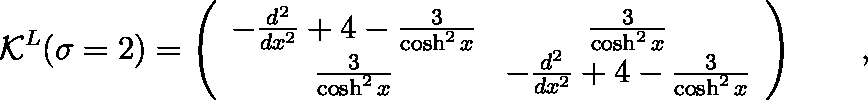
\includegraphics[width=10cm]{latexin}};

\visible<2> {
\node (b)[xshift=6cm, rectangle, scale=0.6, draw,thick,fill=blue!0,text width=32em, rounded corners, inner sep =5pt, minimum height=1em]{\baselineskip=50pt \footnotesize
\sTWO

};
  \path[draw, <-] (b) --  (b -| gal.east);
}
\end{tikzpicture}
  \end{center}
\end{frame}

\begin{frame}{Im2Latex}
\research{\cite{Deng2016} w/ Bloomberg}
\begin{center}
  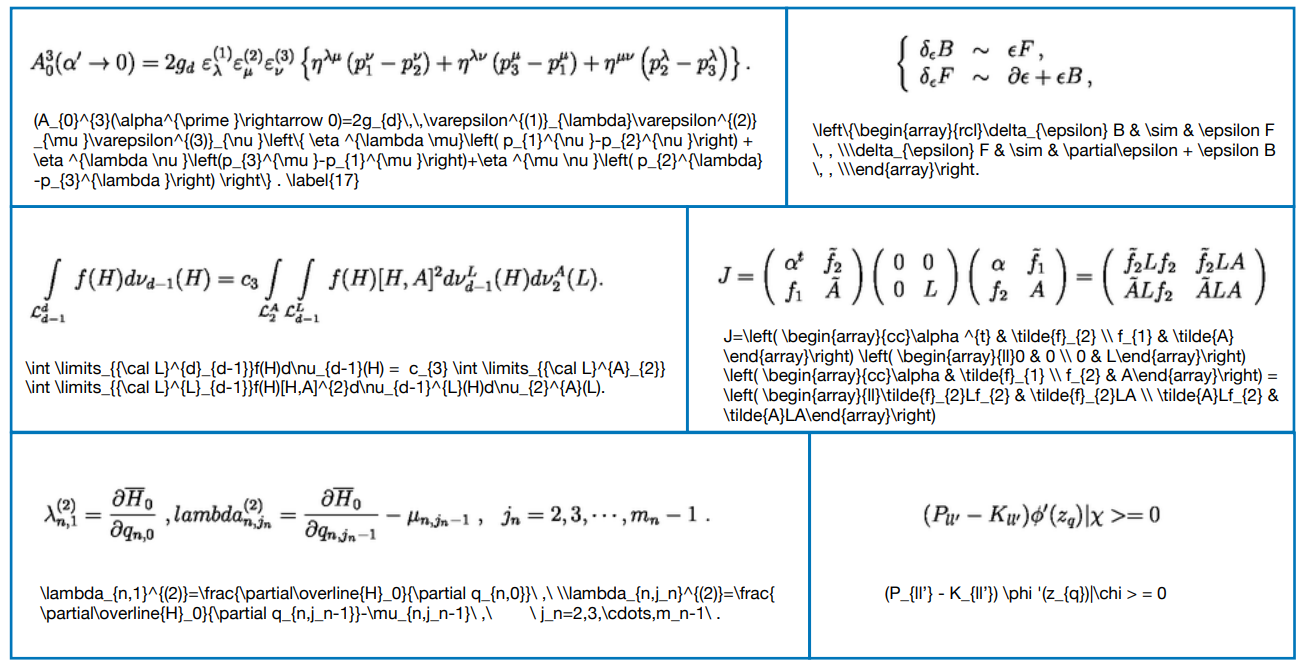
\includegraphics[height =0.75\textheight]{imlatex}
\end{center}
\end{frame}


\begin{frame}{Im2Latex}
\research{\cite{Deng2016} w/ Bloomberg}


  \vspace{-0.25cm}
  \begin{center}
    \movie[width=\textwidth, repeat, height=0.85\textheight, width=\textwidth, poster, showcontrols]{Temporary}{videos/latex.mp4}
  \end{center}

\end{frame}
